\documentclass[nobib]{tufte-handout}

\usepackage[backend = biber, style=apa]{biblatex}
%\addbibresource{../M3_-_Pariser_Kommune.bib}
\usepackage[autostyle]{csquotes}  
%\bibliographystyle{plain}
\usepackage{hyphenat}
%\renewcommand{\cite}[2][0pt]{\sidenote[][#1]{\fullcite{#2}}}
\renewcommand{\cite}[2][0pt]{\sidenote[][#1]{\parencite{#2}}}

% Hyperlinks
%\usepackage[colorlinks,citecolor=red,urlcolor=blue,bookmarks=false,hypertexnames=true]{hyperref}
% No paragraph indentation!
\setlength{\parindent}{0in}
% Micro font adjustments
\usepackage{microtype}
% Epigraph type quotes
\usepackage{epigraph}
% Images
\usepackage{graphicx}
%\graphicspath{ {C:/Users/demir/images/} }
% Boxes around texts
\usepackage{tcolorbox}
% Enumerate
\usepackage{enumerate} 

% call this one with wbox
\newtcolorbox{whitebox}[2][]{standard jigsaw, opacityback=0, title={#2}, 
colbacktitle=white!,
coltitle=Black
}

\begin{document}
\title{Working with Text Data | Basic definitions}
\maketitle

\blockquote{The goal is to amplify reading}
\section{Possible types of strings}%
\label{sec:possible_types_of_strings}

\begin{itemize}
    \item Categorical Data

    \item Free strings that can be (semantically) mapped to categories

    \item Structured string data

    \item Text data
\end{itemize}


\section{Typology}%
\label{sec:typology}

\begin{itemize}
    \item [\textbf{Corpus}] A dataset of \textit{documents}

    \item [\textbf{Document}] A single data point in corpus, a single text.
\end{itemize}

\section{Definitions}%
\label{sec:definitions}

\begin{itemize}
    \item [ \textbf{bag-of-words}] A text that reduced only to the count of how often the words appear in it after discarding the structure (chapters, paragraphs, sentences, formatting etc.) in it.

    \item [\textbf{tokenization}] Split each document into the words that appear in it (tokens).

    \item [\textbf{vocabulary building}] create a vocabulary of all unique words appear in any of the documents and order them (for example alphabetically).

    \item [\textbf{encoding}] For each document, count how often each of the words in vocabulary appear in that document.
\end{itemize}

\begin{marginfigure}
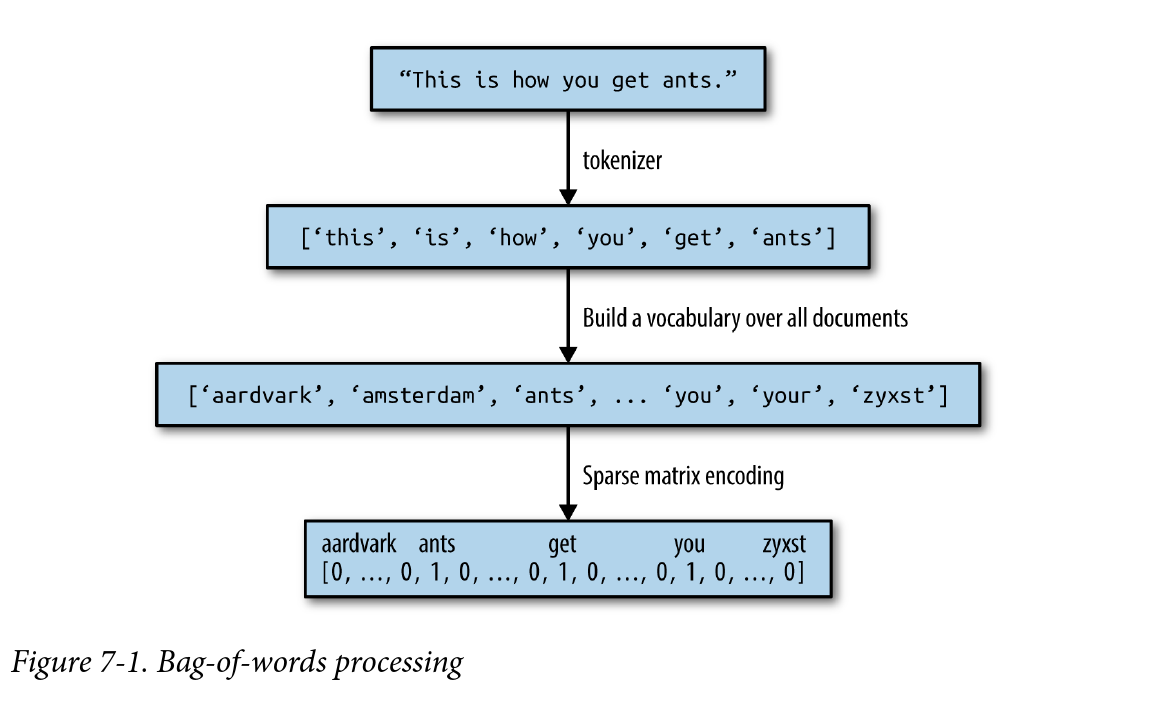
\includegraphics[width=250]{bagofwords_processing.png}
\label{}
\end{marginfigure}



\section{Rescale with tf-idf}%
\label{sec:rescale_with_tf_idf}


\begin{equation}
\operatorname{tfidf}(w, d)=\operatorname{tf} \log \left(\frac{N+1}{N_{w}+1}\right)+1
\end{equation}

\begin{itemize}
    \item [$N$] Number of documents

    \item [$N_{w}$] Number of documents word \(w\) is appearing in.

    \item [$tf$] Number of \(w\) occurences in the specific document we are transforming.
\end{itemize}


\section{n-Grams and the shortcomings of bag-of-words}%
\label{sec:n_grams_and_the_shortcomings_of_bag_of_words}

The main disadvantage of the bag-of-words approach is that it is completely overlooking the order of words, the structure of the text. \footnote{ \textit{it's bad, not good at all} == \textit{it's good, not bad at all}  }. n-Grams (bigrams, trigrams ...) approach is trying to solve this problem.

This feature can be applied by defining \verb|ngram_range| in \verb|CountVectorizer| or \verb|TfidfVectorizer|.
\printbibliography
\end{document}
